%\usepackage{amsmath} % Per le formule matematiche
%\usepackage{adjustbox} % Per la gestione delle tabelle

\chapter{Algoritmi e strutture dati}

\section{Struttura del progetto}
L’applicazione, scritta in linguaggio Java, segue il pattern MVC (Model View Controller), quindi divide la struttura software in tre parti principali: model, view e controller. L’applicazione sfrutta il pattern DAO (Database Access Object) che separa la logica di accesso ai dati dalla logica di business.

Il progetto dell’applicazione è disponibile nel repository Github al seguente link: \url{https://github.com/TdP-prove-finali/LapadulaMarioFrancescoPio}.

Il progetto si compone di tre package:
\begin{itemize}
    \item \textbf{db}: contiene le classi utili all’accesso al DB e all’estrazione dei dati;
    \item \textbf{model}: contiene le classi simulative e le classi che definiscono le proprietà degli oggetti utilizzati nella simulazione. Nel model sono memorizzati tutti i dati della simulazione tramite apposite strutture dati;
    \item \textbf{SimulazioneF1}: contiene le classi controller che gestiscono i fogli FXML e, di conseguenza, la GUI (Graphical User Interface).
\end{itemize}

\section{Software utilizzati}
L’applicazione è stata realizzata tramite l’IDE Eclipse. Per la realizzazione di parte dell’interfaccia grafica è stato utilizzato il software SceneBuilder. Il DBMS utilizzato è MariaDB con interfaccia grafica HeidiSQL.

\section{Strutture dati}
La maggior parte dei dati è estratta dal DB e memorizzata in HashMap. Nel model, per la memorizzazione temporanea, sono utilizzati anche LinkedList e ArrayList. Nelle classi dedicate alla simulazione, i tempi in gara e le varie classifiche dei punteggi sono memorizzate e aggiornate tramite HashMap.

\section{Algoritmi simulativi}

\subsection{Simulatore generale}
L’applicazione utilizza un algoritmo di simulazione a eventi discreti. Ci sono tre classi dedicate alla simulazione di eventi: la principale è \texttt{Sim}, che si occupa di amministrare la simulazione dei vari eventi durante l’intera stagione. Durante l’inizializzazione del simulatore principale viene creata una coda di eventi di tipo Sessione. Per ogni circuito presente nella struttura dati fornita, vengono creati due oggetti Sessione: uno di tipo ‘Qualifica’ e uno di tipo ‘Gara’. La classe \texttt{Sim} usa due sottoclassi per simulare nello specifico i vari tipi di eventi: alla classe \texttt{SimQ} sono passate le Sessioni di tipo ‘Qualifica’ e alla classe \texttt{SimR} quelle di tipo ‘Gara’.
\\[3ex]

\begin{figure}[h!]
    \centering
    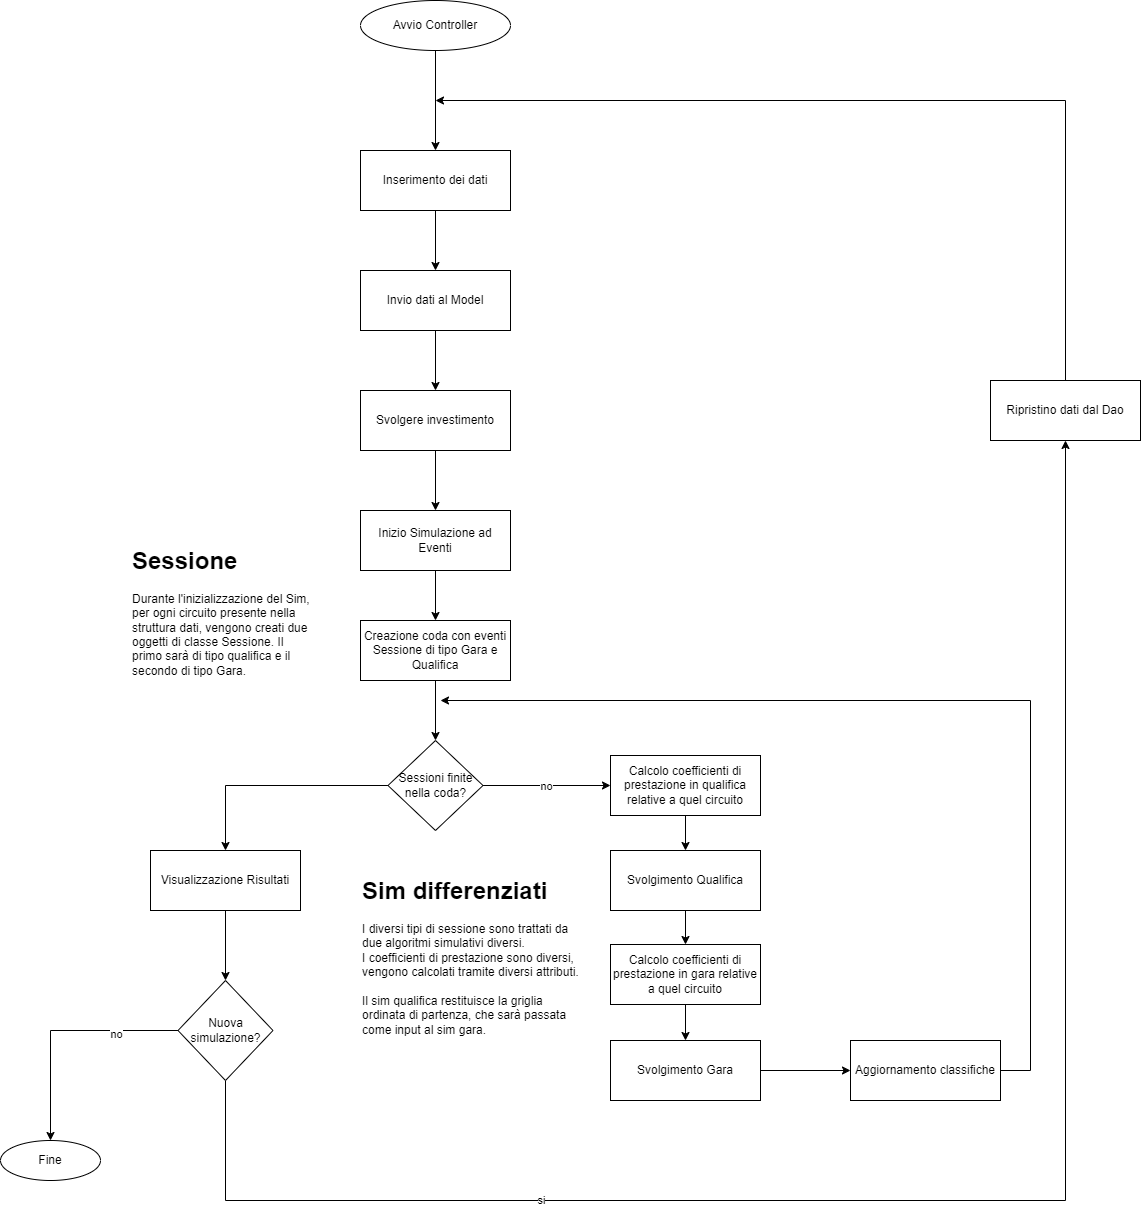
\includegraphics[width=0.8\linewidth, height=11.5cm]{Figures/garaU.png}
    \caption{Flow chart esplicativo riguardo il funzionamento del simulatore generale}
    \label{fig:flowchart_simulatore_generale}
\end{figure}
\newpage
\subsection{Simulatore qualifica}
Alla classe SimQ vengono passati nel costruttore la lista dei piloti partecipanti alla Sessione e l’oggetto Track che indica il circuito su cui viene svolta la sessione.

Il simulatore SimQ ha il compito di calcolare la griglia di partenza per la gara, per poi restituirla alla classe Sim. La griglia viene calcolata confrontando e ordinando degli indici di prestazione relativi ad ogni pilota.

Questi indici sono calcolati all’inizio di ogni sessione attraverso la combinazione dei seguenti fattori:
\begin{itemize}
    \item valore di prestazione della vettura del pilota su quel determinato circuito, calcolato mediante l’algoritmo \texttt{CalcolaPrestazioneScuderia()};
    \item valore di overall totale del pilota;
    \item fattore casuale ottenuto campionando una distribuzione normale.
\end{itemize}

Questi fattori sono poi moltiplicati per delle costanti relative e sommati tra loro per ricavare l’indice di prestazione finale. Successivamente la griglia di partenza viene stilata classificando in ordine decrescente gli indici ottenuti dai piloti.


\subsection{Simulatore gara}
Ricavata la griglia di partenza per la gara, viene fornita al costruttore della classe SimR tramite una lista ordinata di oggetti di tipo Pilota. Prima di iniziare la simulazione delle varie fasi della gara, vi è il calcolo degli indici di prestazione relativi alla gara, diversi da quelli usati nel SimQ per stilare la griglia.

L’indice di prestazione di gara è un valore calcolato attraverso la combinazione dei seguenti fattori:
\begin{itemize}
    \item valore di prestazione della vettura del pilota su quel determinato circuito, calcolato mediante l’algoritmo CalcolaPrestazioneScuderia();
    \item valore di overall totale del pilota;
    \item fattore casuale ottenuto campionando una distribuzione normale;
    \item valore delle caratteristiche Smoothness e Control del pilota moltiplicati per l’indice di consumo gomma in quel circuito;
    \item valore della caratteristica Adaptability del pilota, solo in caso di gara disputata in condizioni di pioggia.
\end{itemize}

Questi fattori sono poi moltiplicati per delle costanti relative e sommati tra loro per ricavare l’indice di prestazione finale. Gli indici saranno poi utilizzati per calcolare il tempo sul giro di un pilota per ogni giro di gara. Calcolati gli indici, si procede simulando il momento della partenza e poi simulando lo svolgimento di ogni giro fino alla fine della gara.

Il tempo di percorrenza di un giro di un pilota è calcolato mediante delle operazioni tra l’indice di prestazione e un fattore casuale campionato da una distribuzione normale.

Durante ogni giro potrebbero capitare imprevisti ad un pilota, come un guasto alla vettura o un incidente in gara, che lo costringerebbero a ritirarsi dalla corsa. L’evento del guasto alla vettura è gestito da un indice di successo probabilistico dipendente dal valore tecnico di Affidabilità della vettura del pilota. Invece l’evento ‘incidente in gara’ è gestito da un indice di successo probabilistico dipendente dalla combinazione dalle caratteristiche Adaptability, Control, Reactions e Aggressivity del pilota.

Prima della fine di ogni giro (dal quarto giro in poi) viene data ai piloti la possibilità di sorpassare se il distacco dal pilota davanti è inferiore a un secondo. In questo caso viene richiamato un algoritmo che stabilirà se il pilota dietro tenterà il sorpasso e se riuscirà nel suo tentativo. Durante un sorpasso, la probabilità che uno o entrambi i piloti coinvolti facciano incidente è più alta della norma e, di conseguenza, che si ritirino dalla gara.

Alla fine di ogni giro vengono poi aggiornati i distacchi tra i piloti in gara. Durante la gara, ogni pilota deve rientrare ai box per un pit stop per due volte. Il tempo perso durante un pit stop viene calcolato tramite operazioni tra i seguenti fattori:
\begin{itemize}
    \item tempo medio di pit stop della scuderia del pilota;
    \item valore qualitativo della Pit Crew della scuderia del pilota;
    \item tempo di percorrenza della pit lane del circuito;
    \item fattore casuale campionato da una distribuzione normale.
\end{itemize}

Per gestire il tempismo dei pit stop, si usa una variabile ‘Stint’ calcolata nel seguente modo:
\[ Stint = \left\lfloor \frac{NGiriGara + 3}{NPitStop + 1} \right\rfloor \]


\begin{figure}[H]
    \centering
    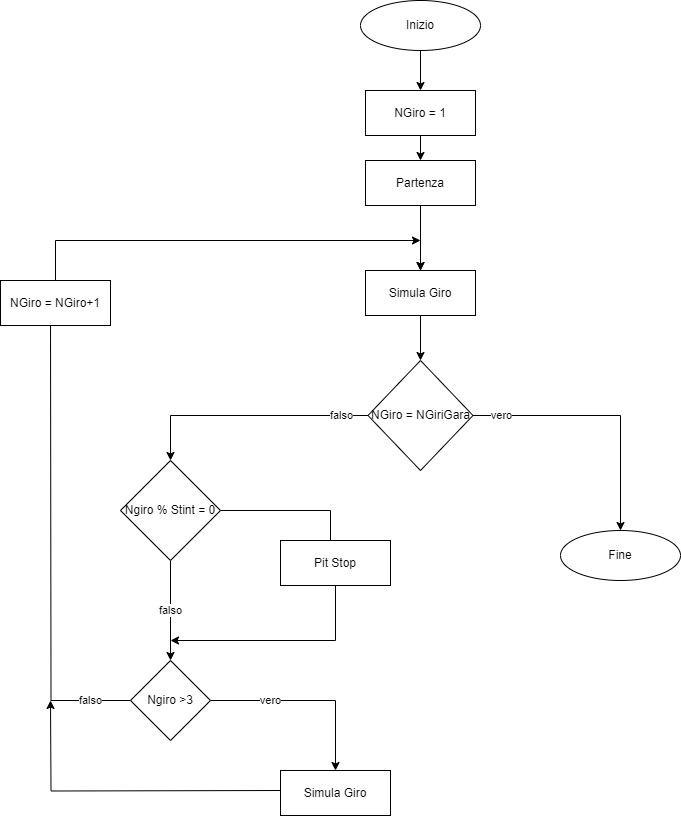
\includegraphics[width=0.8\linewidth, height=9cm]{Figures/gara.png}
    \caption{Flow chart esplicativo riguardo le procedure della simulazione di una gara}
    \label{fig:flowchart_simulatore_gara}
\end{figure}

\subsection{Simulatore sorpasso}
Come riportato nel Capitolo 5.4.3, un sorpasso può verificarsi solo quando il distacco tra due piloti è inferiore a un secondo. L’algoritmo per simulare un sorpasso si divide in due fasi. Un algoritmo preliminare stabilisce in base a un indice di successo probabilistico se il pilota tenterà o meno il sorpasso. Questa variabile dipende dai seguenti fattori:
\begin{itemize}
    \item fattore casuale campionato da una distribuzione normale;
    \item valore della caratteristica Aggressivity del pilota;
    \item indice di probabilità di sorpasso del circuito.
\end{itemize}
Se l’algoritmo restituisce un esito positivo, si aziona un secondo algoritmo che stabilirà l’esito del tentativo di sorpasso. Questo algoritmo prende in analisi le caratteristiche dei due piloti in azione, nello specifico:
\begin{itemize}
    \item overall totale, indice di prestazione della scuderia, valore della caratteristica Defending per il pilota che deve difendersi dal sorpasso; 
    \item overall totale, indice di prestazione della scuderia, valore della caratteristica Overtaking per il pilota che deve effettuare il sorpasso.
\end{itemize}
Questi dati vengono combinati con fattori casuali e poi confrontati per stabilire l’esito della manovra.


\begin{figure}[h!]
    \centering
    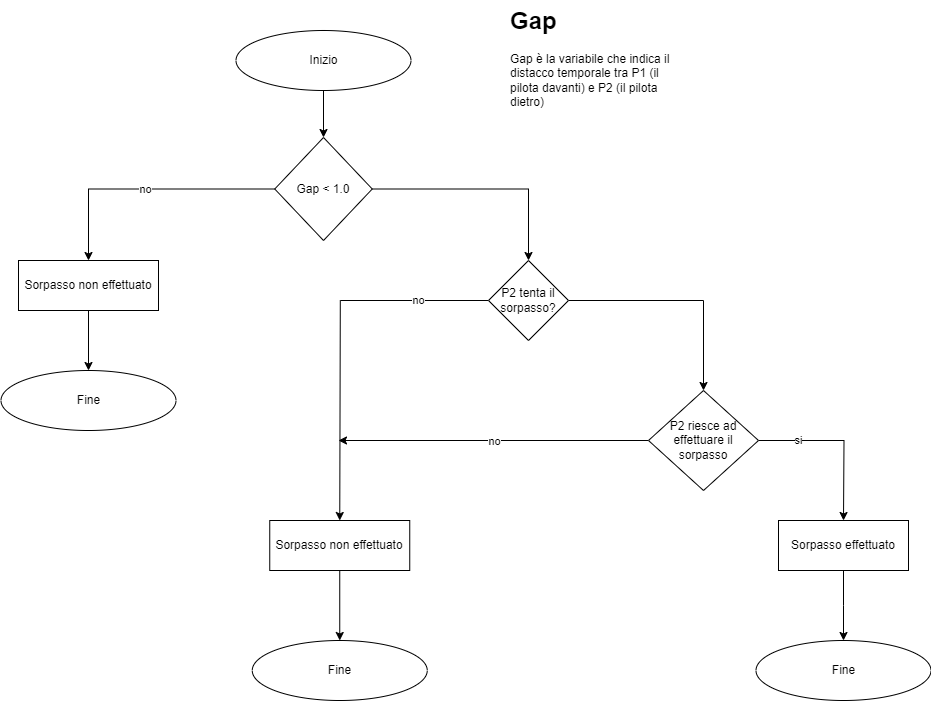
\includegraphics[width=0.8\linewidth]{Figures/Sorpasso1.png}
    \caption{Flow chart esplicativo riguardo il funzionamento dell’algoritmo simulativo per l’azione di sorpasso}
    \label{fig:flowchart_simulatore_sorpasso}
\end{figure}

\subsection{Utilizzo di casualità negli algoritmi}
Nella simulazione sono stati utilizzati fattori randomici per simulare diversi tipi di eventi possibili, come l’azione di sorpasso, la simulazione del tempo sul giro, la partenza della gara, il tempo impiegato per un pit stop e le prestazioni individuali dei piloti in qualifica e in gara. L’utilizzo di questa aleatorietà aiuta a modellare l'incertezza, la variabilità naturale e la complessità di fenomeni che non possono essere descritti completamente da modelli deterministici.


